\documentclass[article]{ajs}

%%%%%%%%%%%%%%%%%%%%%%%%%%%%%%
%% declarations for jss.cls %%%%%%%%%%%%%%%%%%%%%%%%%%%%%%%%%%%%%%%%%%
%%%%%%%%%%%%%%%%%%%%%%%%%%%%%%
 
\usepackage{etoolbox}
\usepackage{amsmath}
\usepackage{graphicx}
\graphicspath{{images/}}
 
 
%% almost as usual
\author{Matthias Medl\,\orcidlink{0000-0002-3354-4579}\\ Institute of Statistics \\ BOKU University \\ Vienna \And 
        Dianne Cook\,\orcidlink{0000-0002-3813-7155}\\ Econometrics and Business Statistics \\ Monash University \\ Melbourne \And
        Ursula Laa\,\orcidlink{0000-0002-0249-6439}\\ Institute of Statistics \\ BOKU University \\ Vienna}
%% \AND can be used instead of \And and starts a new line
\title{Interactively Visualizing Clustering in Multivariate Data Using pytourr}

%% for pretty printing and a nice hypersummary also set:
\Plainauthor{Matthias Medl, Dianne Cook, Ursula Laa} %% comma-separated
\Plaintitle{Interactively Visualizing Clustering in Multivariate Data Using pytourr} %% without formatting
\Shorttitle{pytourr} %% a short title (if necessary)

%% an abstract and keywords
\Abstract{
Lorem ipsum Lorem ipsum Lorem ipsum Lorem ipsum Lorem ipsum Lorem ipsum
Lorem ipsum Lorem ipsum Lorem ipsum Lorem ipsum Lorem ipsum Lorem ipsum
Lorem ipsum Lorem ipsum Lorem ipsum Lorem ipsum Lorem ipsum Lorem ipsum
Lorem ipsum Lorem ipsum Lorem ipsum Lorem ipsum Lorem ipsum Lorem ipsum
Lorem ipsum Lorem ipsum Lorem ipsum Lorem ipsum Lorem ipsum Lorem ipsum
Lorem ipsum Lorem ipsum Lorem ipsum Lorem ipsum Lorem ipsum Lorem ipsum
Lorem ipsum Lorem ipsum Lorem ipsum Lorem ipsum Lorem ipsum Lorem ipsum
Lorem ipsum Lorem ipsum Lorem ipsum Lorem ipsum Lorem ipsum Lorem ipsum
}
\Keywords{interactive graphics, tourr, exploratory data analysis, \proglang{R}, \proglang{python}}
\Plainkeywords{keywords, comma-separated, non-capitalized,, R} %% without formatting
%% at least one keyword must be supplied

%% publication information
%% NOTE: Typically, this can be left commented and will be filled out by the technical editor
%% \Volume{50}
%% \Issue{9}
%% \Month{June}
%% \Year{2012}
%% \Submitdate{2012-06-04}
%% \Acceptdate{2012-06-04}
%% \setcounter{page}{1}
\Pages{1--xx}

%% The address of (at least) one author should be given
%% in the following format:
\Address{
  Matthias Medl\\
  Institue of Statistics\\
  BOKU University Vienna\\
  E-mail: \email{matthias.medl@boku.ac.at}\\
}
%% It is also possible to add a telephone and fax number
%% before the e-mail in the following format:
%% Telephone: +43/512/507-7103
%% Fax: +43/512/507-2851

%% for those who use Sweave please include the following line (with % symbols):
%% need no \usepackage{Sweave.sty}

%% end of declarations %%%%%%%%%%%%%%%%%%%%%%%%%%%%%%%%%%%%%%%%%%%%%%%


\begin{document}

\section{Introduction}

\begin{itemize} \itemsep 0in
\item Background to clustering analysis
\item Visualising clusters, including tours
\item Difference between clustering and partitioning
\item How do you know whether the results are useful
\end{itemize}

\section{Related Work}

Previous attempts have been made to bring interactivtiy to the tourr package. The galahr package \citep{galahr} was an attempt to so by means of the R packages shiny \citep{shiny} and plotly \citep{plotly}, but ultimately suffered from performance issues when the size of the investigated dataset became too large (n>10 000). To overcome these issues, the detourr package \citep{detourr}, which precomputes multiple projections in R and subsequently visualizes them in an interactive display using Javascript, has been developed. While detourr showed better performance, the interactivtiy is still limited as only precomputed projections can be displayed and there is no option to show multiple linked displays simultaneously. The mmtour package \citep{laa2023new} is a \proglang{Mathamatica} implementation allowing for interaction with manual and slice tours.  

\section{The pytourr package}

\subsection{Overview}

The primary objective of this work is to develop an R package that integrates high-performance interactivity through Python packages, such as \texttt{TKinter} \citep{lundh1999introduction}, \texttt{CustomTKinter} \citep{schimansky24}, and \texttt{matplotlib} \citep{Hunter:2007}, with the tourr package \citep{tourr}. This integration is achieved via \texttt{reticulate} \citep{reticulate}, a framework that facilitates seamless interoperability between Python and R.

At the core of the \texttt{pytourr} package is a graphical user interface (GUI) designed to display multiple linked visualizations concurrently. Users can interact with one of the plots, for example, by subselecting specific data points, and the other linked plots will dynamically update to reflect these modifications. This interconnected functionality allows for efficient and immediate analysis of high-dimensional datasets without necessitating extensive coding, thereby streamlining the exploratory data analysis process.

In addition to this core functionality, \texttt{pytourr} offers a variety of interactive plot types, providing users with the flexibility to visualize their data from multiple perspectives. The ability to navigate through various projections of the displayed tours directly within the GUI enables users to explore different aspects of the dataset with ease. Furthermore, users can initiate new tours directly from the interface. The GUI also supports interactive feature selection, allowing users to specify which subset of features should be visualized in the plots. Once users have identified interesting views or settings, \texttt{pytourr} allows them to save the displayed projections, subsets, and plots. This functionality ensures that analysis states can be preserved for further examination or reporting, making the package particularly useful for iterative analysis where findings may need to be revisited or shared with collaborators.

With its high level of interactivity, performance, and ease of use, \texttt{pytourr} streamlines the exploration of complex datasets, offering a powerful tool for researchers working with high-dimensional data.


\subsection{The graphical user interface}

The \texttt{pytourr} GUI can be launched using the function \texttt{interactive\textunderscore tour()}. At a minimum, the user needs to provide both the dataset and the instructions for constructing the desired plots. The dataset must be supplied as a \texttt{data.table}, while the plotting instructions should be passed as a list containing the named elements \texttt{type} and \texttt{obj}. The \texttt{type} element specifies the type of display to generate, such as "scatter" for a scatterplot or "2d\textunderscore tour" for a 2-dimensional tour. The \texttt{obj} element further defines the properties of the chosen display. For example, to create a 2-dimensional tour, the user must provide a \texttt{tour\textunderscore history} object, which can be generated using the \texttt{tourr} package. For a scatterplot, the user needs to provide a vector of strings specifying the names of the features to be displayed. The user can optionally specify the feature names, the arrangement of the plots, predefined subsets of the data (e.g., cluster solutions), custom names for these subsets, the number of available subsets, and the size of each plot.

The GUI is divided into two main sections: a sidebar on the left, which contains a comprehensive set of interactive controls to customize and interact with the displays, and the display area on the right. An overview of the GUI can be seen in figure x.

At the top of the sidebar, users can select and deselect features via checkboxes, determining which features are displayed in the plots. Below this, each subset of the data has a corresponding checkbox, which is used to select the active subset. When a subset is selected, any data points marked in the plots will be moved to this active subset and be colored accordingly. The colored boxes next to the subset names indicate how the datapoints within each subset are colored. Users can adjust the transparency of each subset by clicking these colored boxes. This can be useful when one wants to highlight one or multiple subsets, for instance when wanting to compare to subsets in particular. The subset selection can be reset to its original state at any time by clicking the "Reset original selection" button.

At the top of the sidebar, users can select and deselect features via checkboxes, controlling which features are displayed in the plots. Below the feature selection, each subset has a checkbox that designates the active subset. When datapoints within the plots are manually selected, they will be moved to the active subset and colored accordingly. The colored boxes next to the subset names indicate the colors that the datapoints within each subset are colored. By clicking these colored boxes, users can adjust the transparency of the datapoints within the corrisponding subet, which is particularly useful for highlighting and comparing specific subsets. The initial subset selection (in case one was provided) can be restored at any time by clicking the "Reset original selection" button.

One can move through the projections of a tour by pressing the arrow keys or by specifying the index of the projection the be displayed and pressing the "Update frames" button. Users can animate the tours by toggling the "Animate" checkbox and specifying a time interval, so that the displays automatically move to the next projections after the specified time interval.

When clicking the "Save projections and subsets" button, a file browser is first launched, allowing users to specify the destination for the output files. These files include a PNG image of the current plots, CSV files containing the projection matrices for all displayed tours, and a mapping of the data points to their respective subsets. Additionally, users can initiate new tours of various directly from the sidebar.


\subsection{R/Python interface}

The majority of \texttt{pytourr} was written in Python, while the R side of the package handles setting up the Python environment within the interactive interface is being run, launching the interactive tour, and generating new tours when initiated through the interface. To incorporate the functionality of the \texttt{tourr} package without translating large portions of its code from R to Python, the \texttt{reticulate} package was used. This approach allows \texttt{pytourr} to automatically benefit from updates to \texttt{tourr}.

However, to reduce inefficiencies caused by cross-language communication and to simplify debugging, \texttt{tourr} functions were only accessed when necessary. Core functionalities, such as performing data transformations using projections, were implemented directly in Python. These transformations are based on well-established mathematical principles and are straightforward to replicate, ensuring they remain stable and efficient.

\subsection{Structure of the Python code}

The central component of the Python code is the \texttt{customTKinter} class \texttt{InteractiveTourInterface}. This class centrally stores attributes related to all plots, such as the dataset, subselections, feature selections, and other shared information. Plot-specific data is organized in dictionaries (the Python equivalent of named lists in R), including the display type, construction instructions, tour projections (only in case of tour displays), color schemes for the displayed data, and, where applicable, the selector and manual projection manipulation classes.

The selector classes handle the behavior when users manually select data points to move them to the active subset. After a selection is made, the selector class updates the centrally stored subselection attribute and ensures all other displays reflect these changes. The manual projection manipulation classes construct the arrows representing the projection axes in the displays and manage the manual adjustment of projections. Users can right-click and drag the arrowheads to modify the projections, after which the class orthonormalizes the projection axes and updates both the projection and the transformed data accordingly.

\subsection{Bit blit}

The implementation of bit blitting was crucial to ensuring fast plot updates and providing a smooth user experience. With bit blit, the static elements of the display, such as the outer frames of the plots, are stored as a background image. When a plot is manipulated, only the affected plot is updated, and within that, only the interactive elements, such as the data points and projection axes in a 2-dimensional tour, are rendered on top of the background image.

In practice, this means that the background, without the interactive elements, must be captured either during initialization or after major updates. The entire plot is first rendered without the interactive elements, the background is then saved, and finally, the plot is redrawn with the interactive elements blended in. Since this process is relatively slow, full updates are only triggered during initialization or after significant changes, such as modifications to the set of active features.


\section{Applications}

The Austrian Vacation Activities \cite{dolnicar2003winter} and the Australian Vacation Activities \cite{cliff2009formative} datasets are used to illustrate the methods.

\subsection{Austrian Vacation Activities dataset}

The Austrian Vacation Activities dataset comprises responses from 2,961 adult tourists who spent their holiday in Austria during the 1997/98 season. Participants were asked to evaluate the importance of 27 different activities during their vacation. The survey categorized responses based on four levels of importance: "totally important," "mostly important," "a bit important," and "not important." For analysis, the responses were binarized: a value of 1 was assigned if the activity was rated as "totally important," and a value of 0 if any of the other categories were selected. The survey was conducted by the Europäisches Tourismus Institut GmbH at the University of Trier and focused exclusively on tourists who did not stay in the country's capital cities.

To gain further insight into the dataset a k-means clustering as described in the book "Market Segmentation Analysis" has been performed \citep{leisch2018market}. Therefore, the function \texttt{stepcclust} of the R package \texttt{flexclust
}\citep{flexclust} with k=6 and nrep=20 was used.

\subsubsection{Feature selection}

The original dataset contains \(p\)=27 features. Some of these features are more informative than others. We only want to keep the most informative ones. Additionally, interacting with the pytourr GUI becomes cumbersome when handling more than \textasciitilde
 15 features, making it necessary to reduce the dimensionality of the dataset. An effective and intuitive way to perform feature selection is by using the heatmap display within pytourr. The heatmap supports three different display metrics for feature selection:

\[
\text{Total Fraction:} \quad \frac{\displaystyle\sum_{i = 1}^{k} \sum_{j = 1}^{p} c_{ij}}{n}
\]
The \textbf{Total Fraction} shows the counts \(c_{ij}\) of the \(i\)-th cluster and \(j\)-th feature, normalized by the total number of observations \(n\).

\[
\text{Intra Cluster Fraction:} \quad \sum_{i = 1}^{k} \sum_{j = 1}^{p} \frac{c_{ij}}{c_{i}}
\]
The \textbf{Intra Cluster Fraction} displays the contribution of each feature within a specific cluster, providing insight into how much a feature contributes to the cluster compared to the overall cluster size \(c_i\).

\[
\text{Intra Feature Fraction:} \quad \sum_{j = 1}^{p} \sum_{i = 1}^{k} \frac{c_{ij}}{c_{j}}
\]
The \textbf{Intra Feature Fraction} highlights how a feature contributes across different clusters relative to the overall importance of that feature \(c_j\).

\begin{figure}[h!]
    \centering
    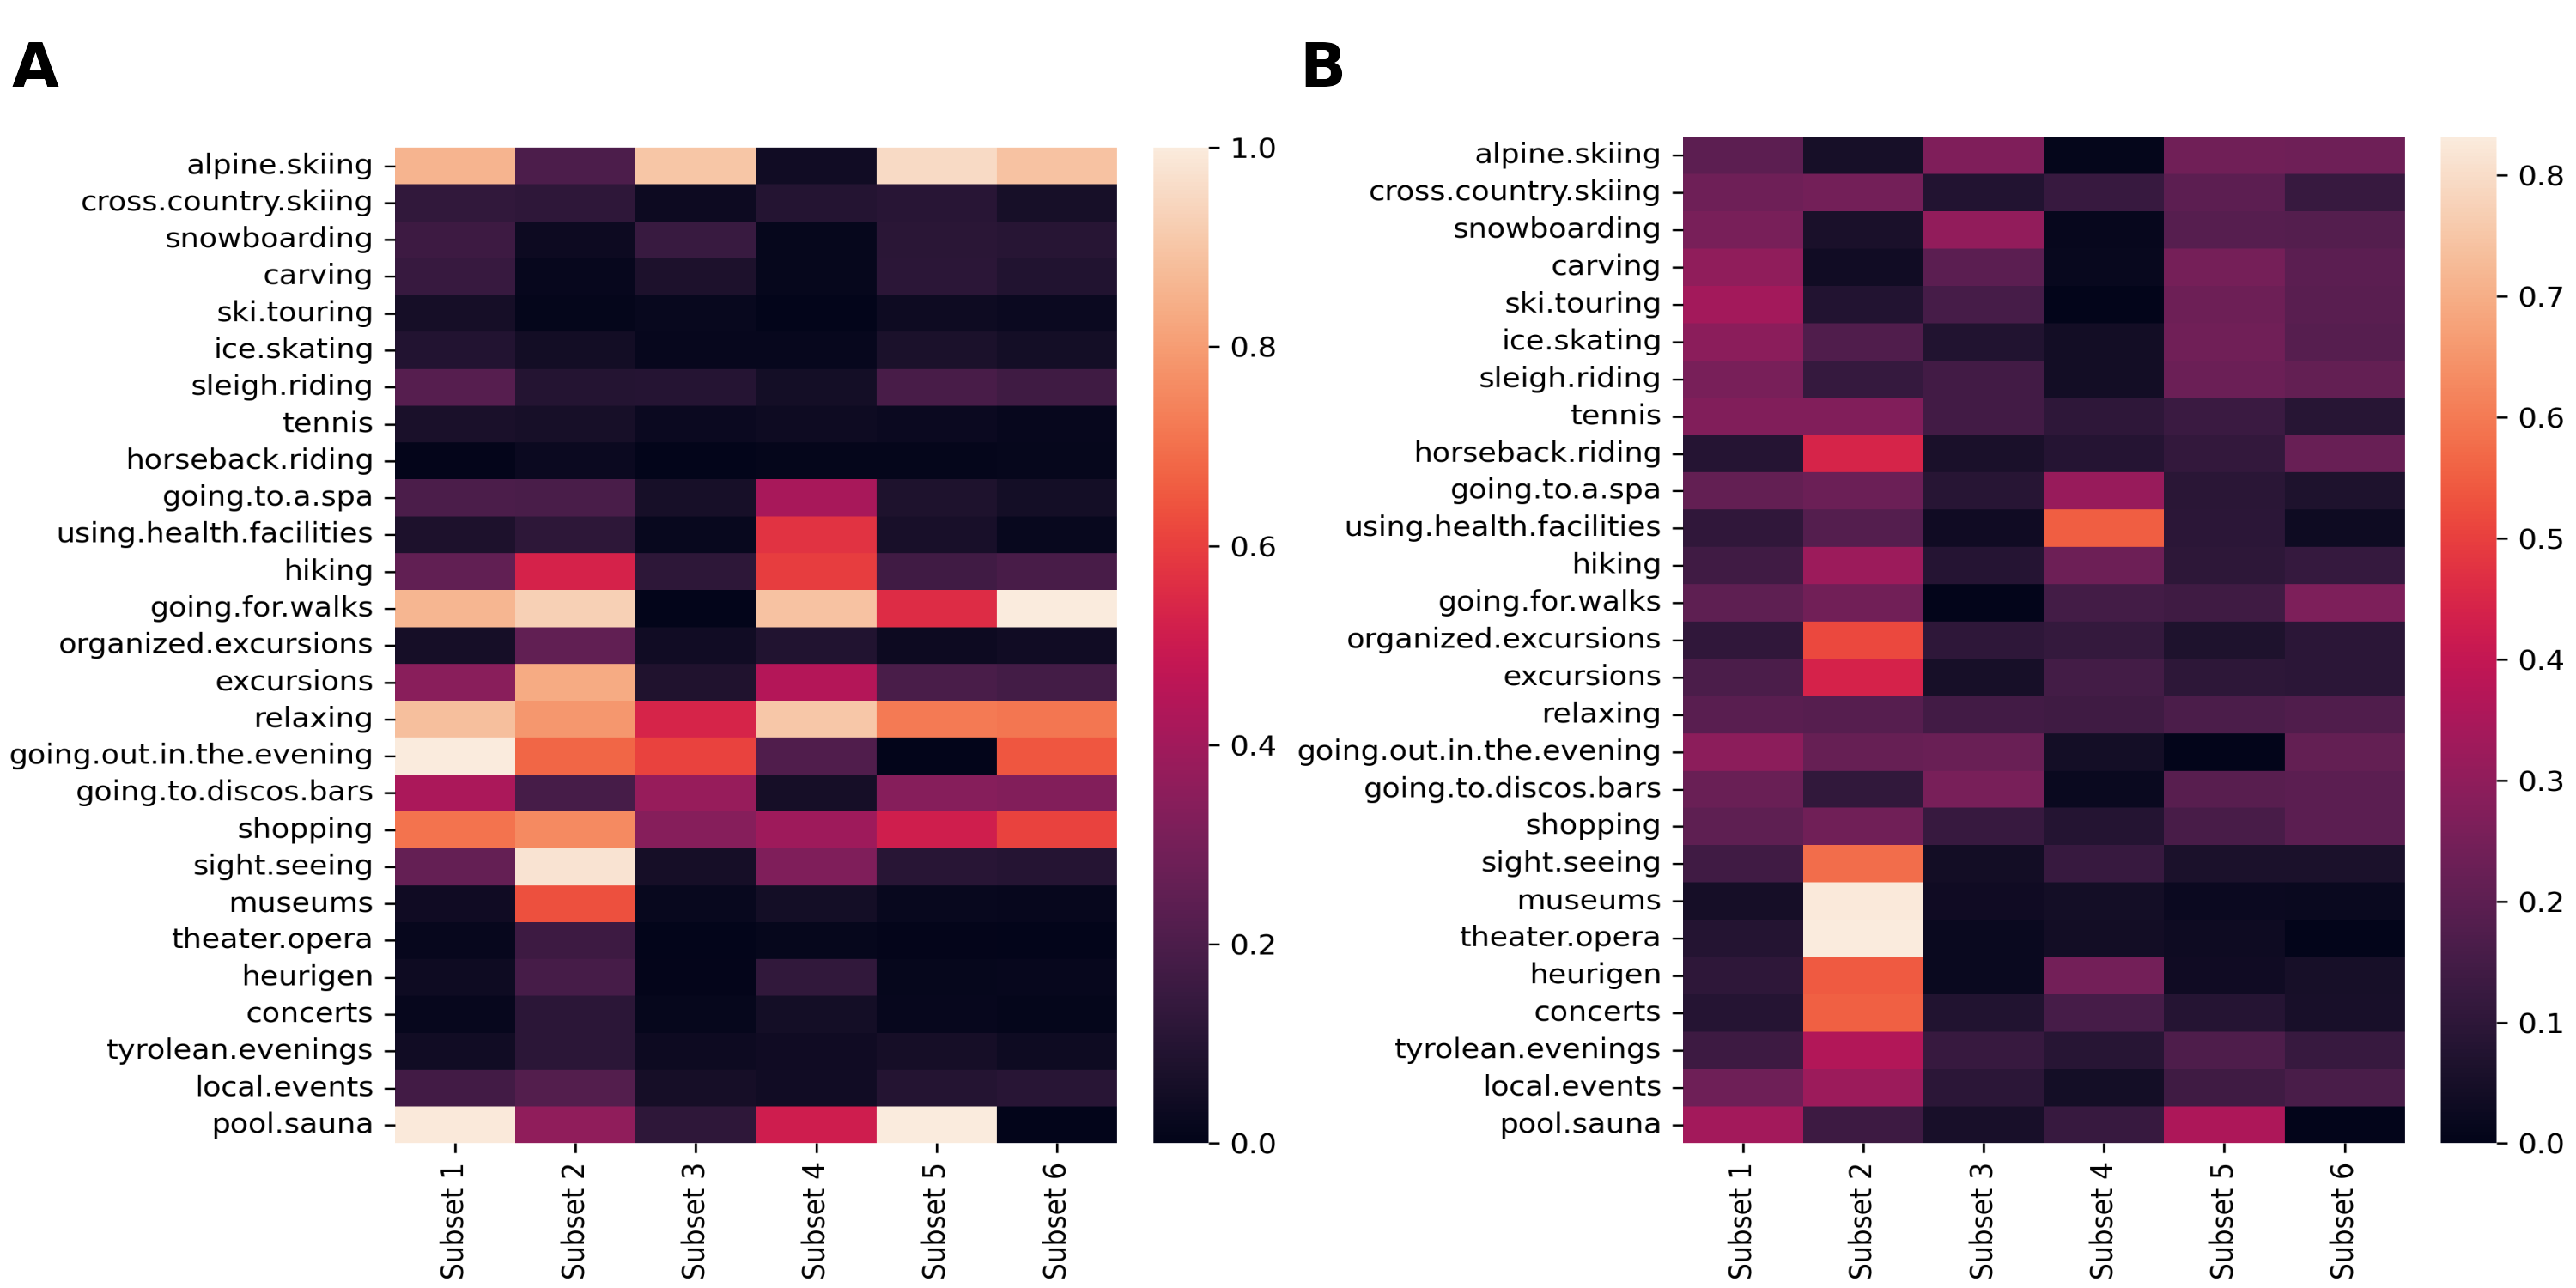
\includegraphics[width=1\textwidth]{winteractiv_heatmap.png}
    \caption{A: heatmap displaying the intra cluster fraction. B: heatmap displaying the intra feature fraction.}
    \label{fig:winteractiv_heatmap}
\end{figure}

In Figure \ref{fig:winteractiv_heatmap}A, we can observe the general interests of tourists within each cluster. For instance, tourists in clusters 1, 3, 5, and 6 predominantly engaged in alpine skiing, while those in clusters 2 and 4 did not. Additionally, we see that activities such as ski touring and horseback riding were generally unpopular across all clusters.

In Figure \ref{fig:winteractiv_heatmap}B, we can determine whether tourists in a particular cluster had a strong preference for certain activities. For example, nearly all tourists who visited museums are grouped in cluster 2, and those who used health facilities are primarily attributed to cluster 4. We can also identify activities that were similarly popular across all clusters, such as relaxing.

By using the heatmap with these metrics, we can perform feature selection by removing unpopular activities and those that were consistently similar across all clusters. After performing the feature selection by unchecking the corresponding checkboxes in the GUI using this strategy, the following 12 activities remained: alpine skiing, going to a spa, using health facilities, hiking, going for walks, excursions, going out in the evening, going to discos/bars, shopping, sightseeing, museums, and pool/sauna.

We can now repeat the k-means clustering with \texttt{stepcclust} on the reduced dataset. Silhouette plots of both cluster solutions can be seen in Figure \ref{fig:silhouette_comparison}. By comparing both silhouette plots, we can see that the cluster solution with the reduced dataset results in a clustering of higher quality. Thus, we will continue with the analysis on the reduced dataset with the corresponsig cluster solution. We can also see in Figure \ref{fig:silhouette_comparison}B that cluster 3 is of comparatively low quality.

\begin{figure}[h!]
    \centering
    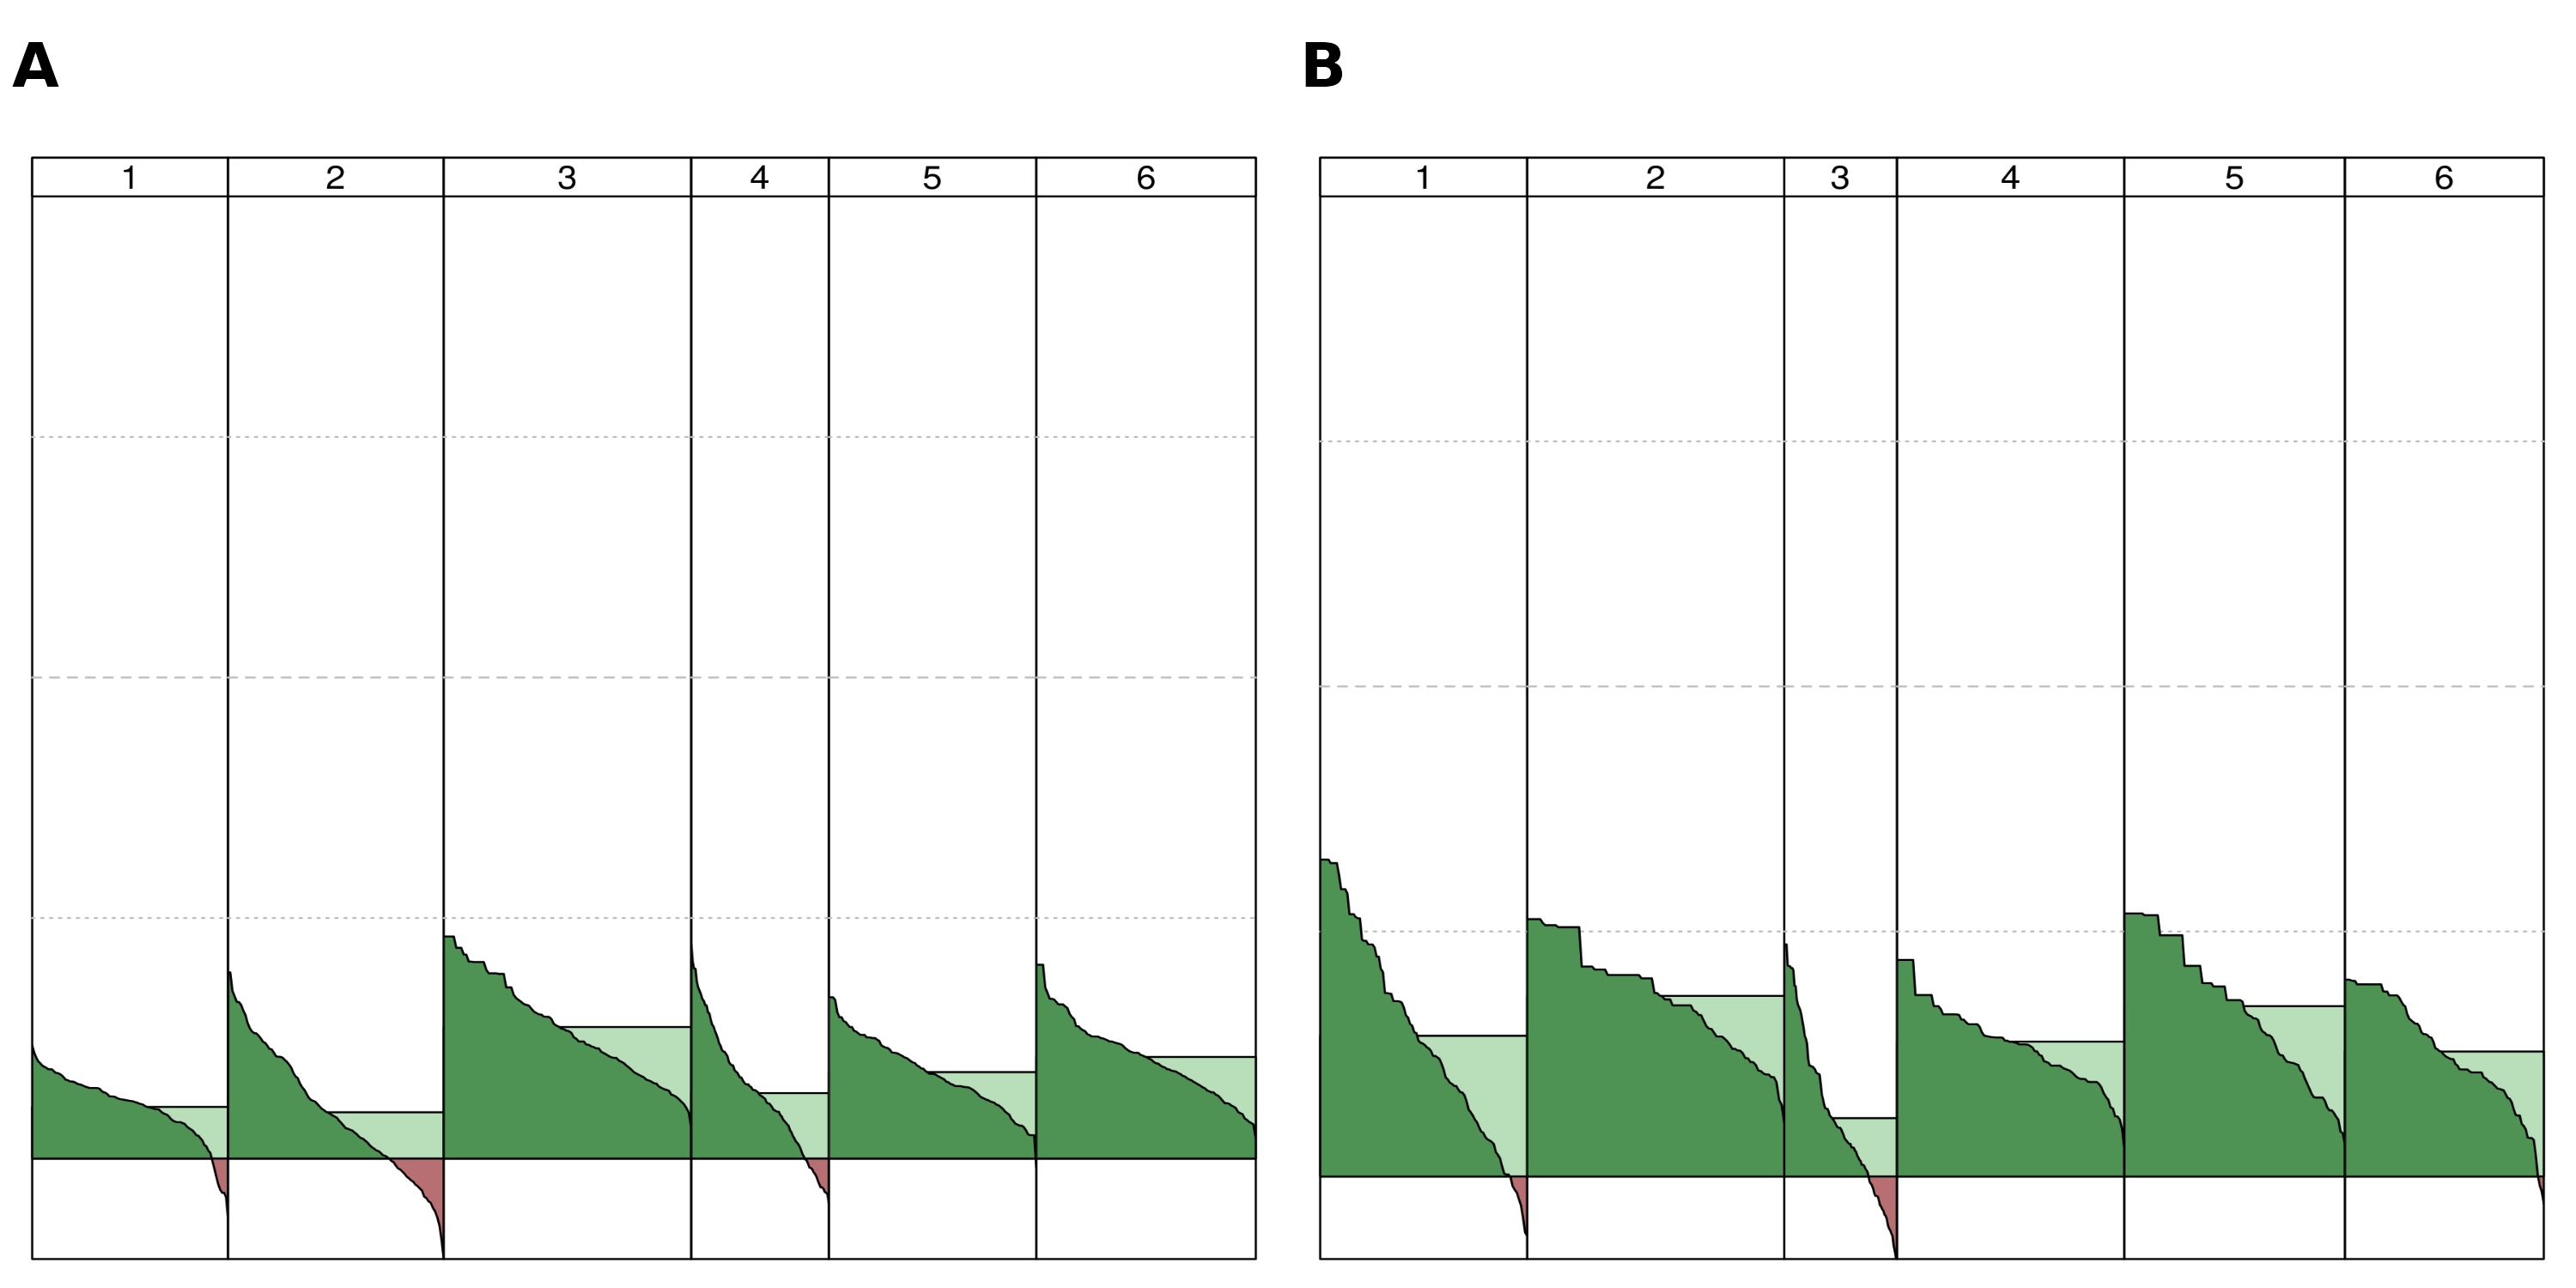
\includegraphics[width=1\textwidth]{silhouette_comparison.png}
    \caption{A: silhouette plot of the k-means solution of the full dataset. B: silhouette plot of the k-means solution with the reduced dataset.}
    \label{fig:silhouette_comparison}
\end{figure}

We can further explore the similarities between the clusters by initializing an \texttt{interactive\_tour()} with a 2D tour based on the linear discriminant analysis (LDA) projection pursuit index. By navigating through the tour, we can observe various projections, and when a projection that separates the clusters is found, we highlight each cluster sequentially. The different highlighted clusters can be seen in Figure \ref{fig:silhouette_comparison}.

\begin{figure}[h!]
    \centering
    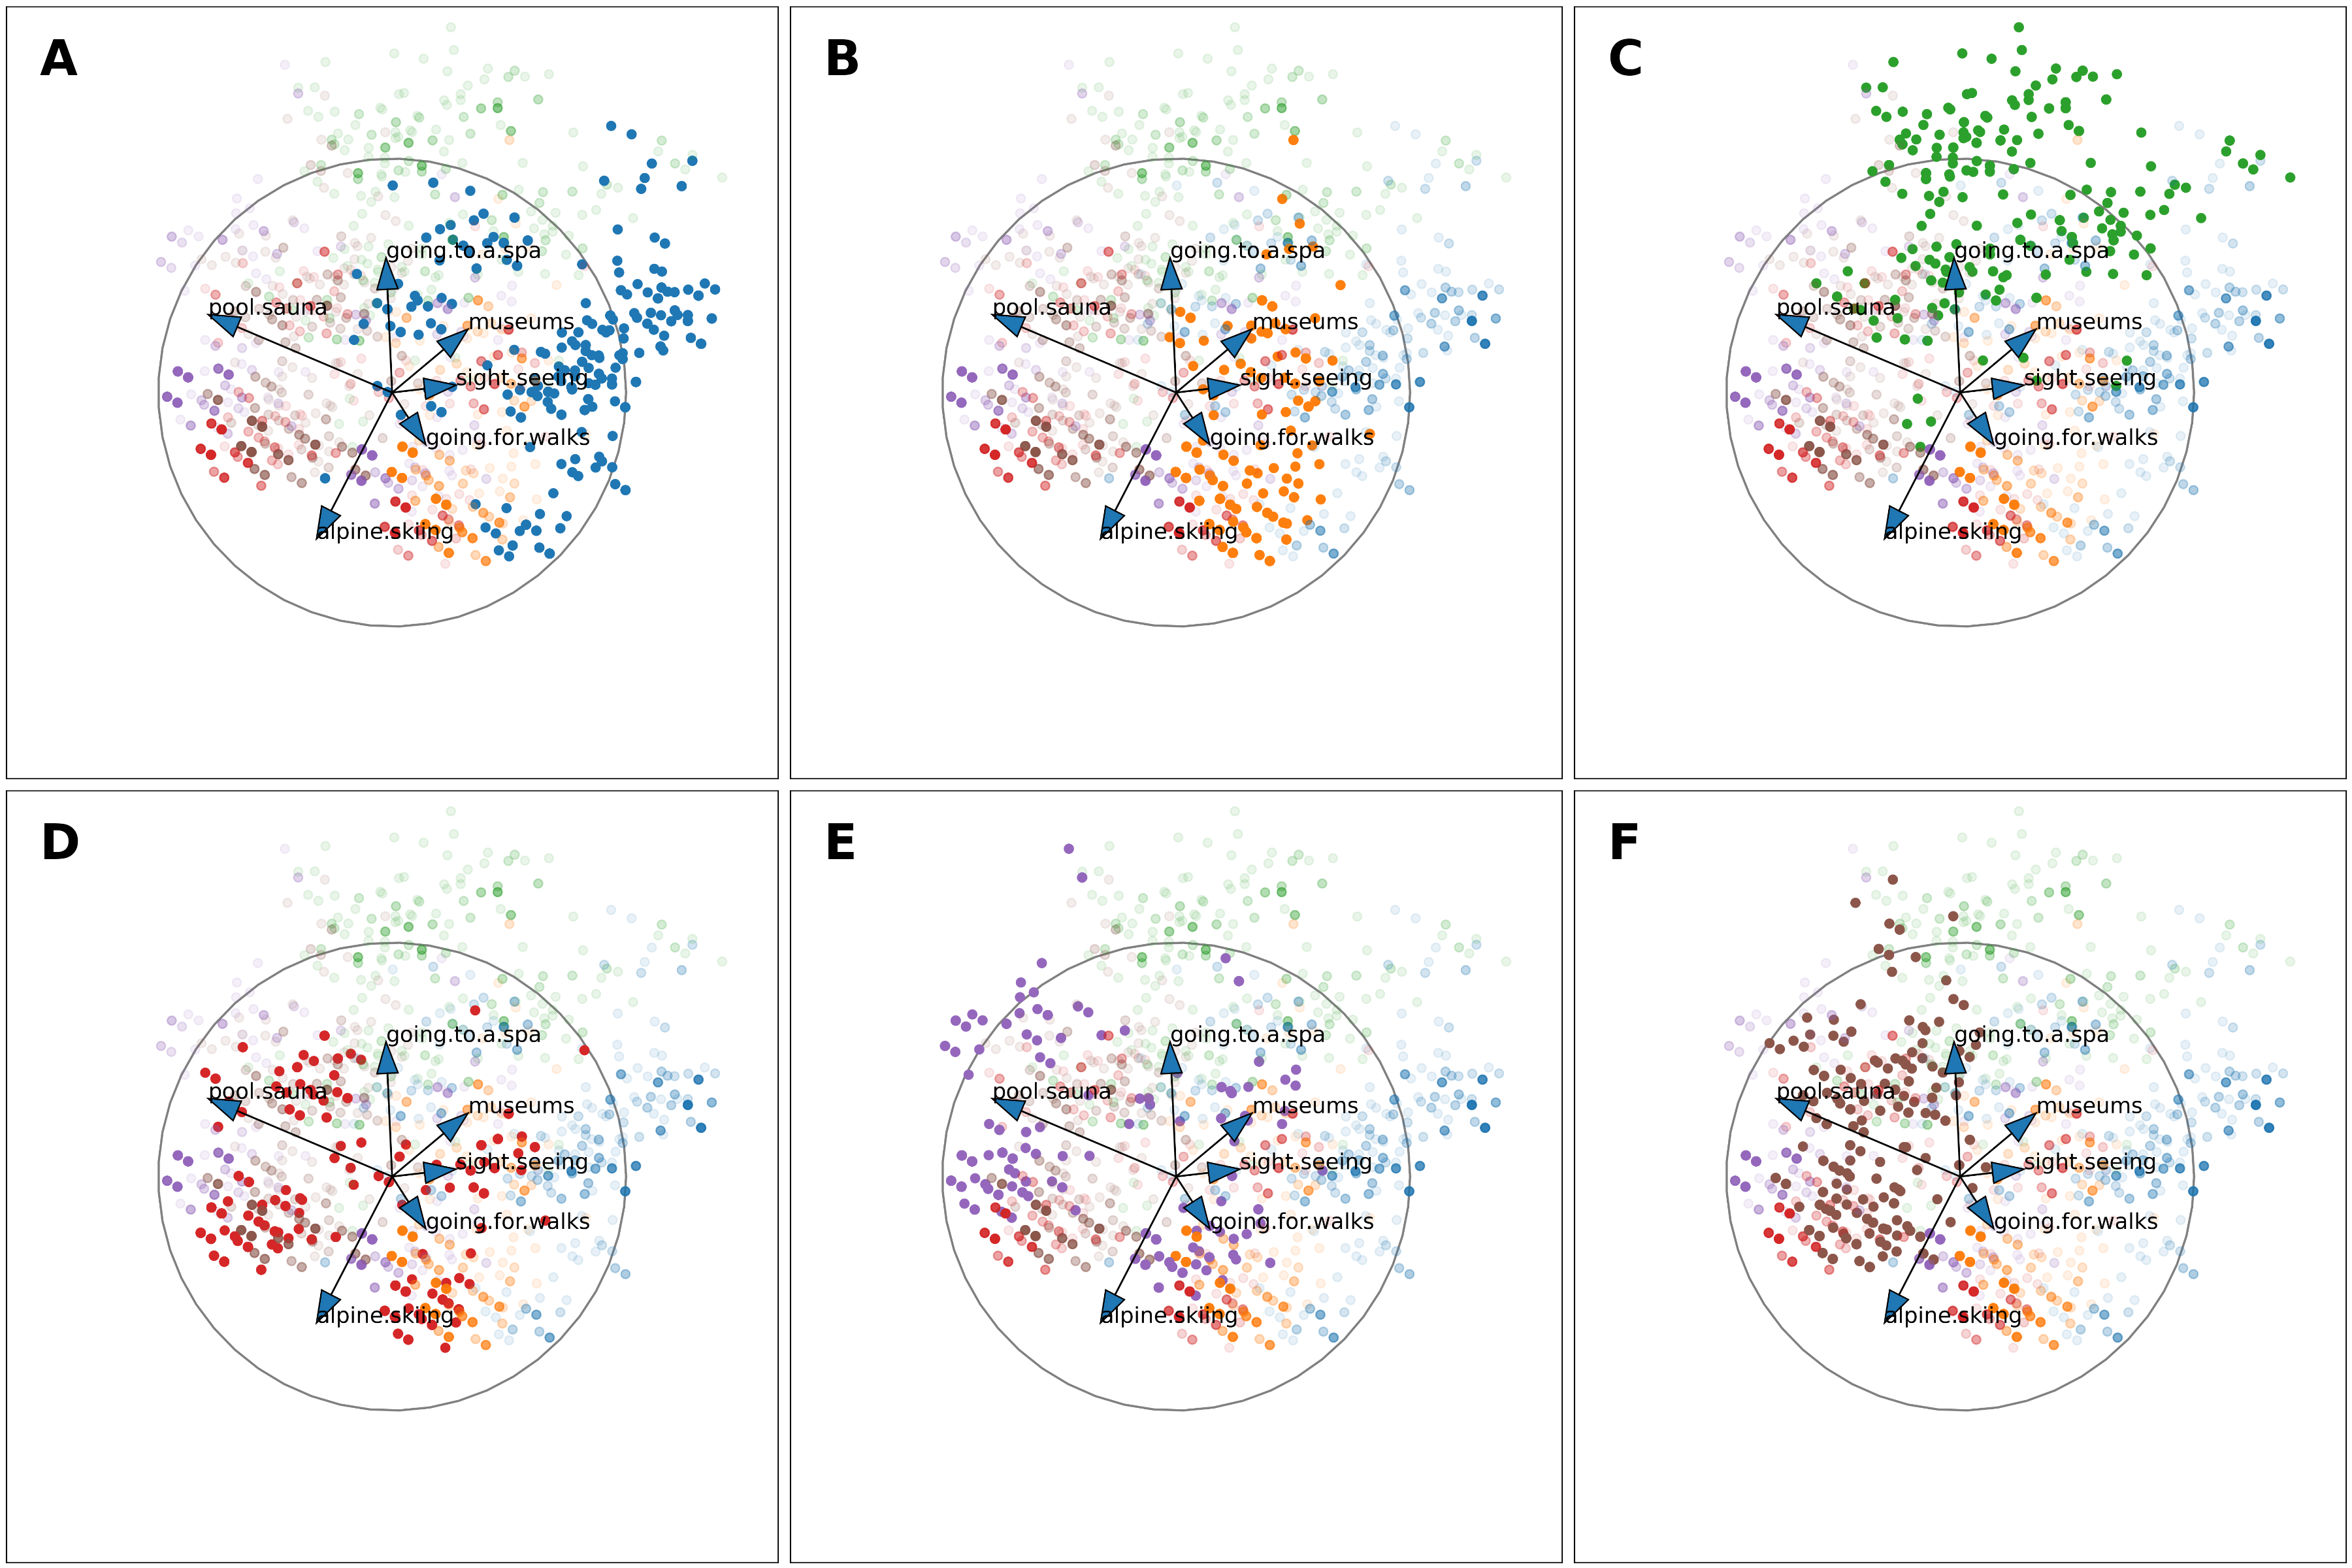
\includegraphics[width=1\textwidth]{winter_activ_cluster_highlights.png}
    \caption{Cluster highlights: \textbf{A} - Cluster 1 (blue), \textbf{B} - Cluster 2 (orange), \textbf{C} - Cluster 3 (green), \textbf{D} - Cluster 4 (red), \textbf{E} - Cluster 5 (violet), \textbf{F} - Cluster 6 (brown).}
    \label{fig:winter_activ_cluster_highlights}
\end{figure}

This process allows us to visually assess the separation and similarities between the clusters, providing insight into the structure of the dataset. By highlighting each cluster individually, we can evaluate their distinctiveness in different projections. The most influential features shown in Figure \ref{fig:winter_activ_cluster_highlights} are pool/sauna, alpine skiing, museums, and going to the spa. The projection roughly separates clusters 1, 2, and 3 from each other and the other three clusters, which appear to be quite similar. 

By manually manipulating the projection axes or initiating a local tour, we can gain further insight into the similarities between the different clusters. This interactive exploration allows for a more nuanced understanding of the relationships between clusters and the influence of key features on the separation of the data.


\subsubsection{Manual cluster improvement}

We have seen in Figure \ref{fig:silhouette_comparison} that clusters 1 and 3 contain some data points that do not fit well into their respective clusters. Manual selection of data points can be employed to further improve the quality of the cluster solution. To do this, we first initialize an \texttt{interactive\_tour()} with the following components:

\begin{figure}[h!]
    \centering
    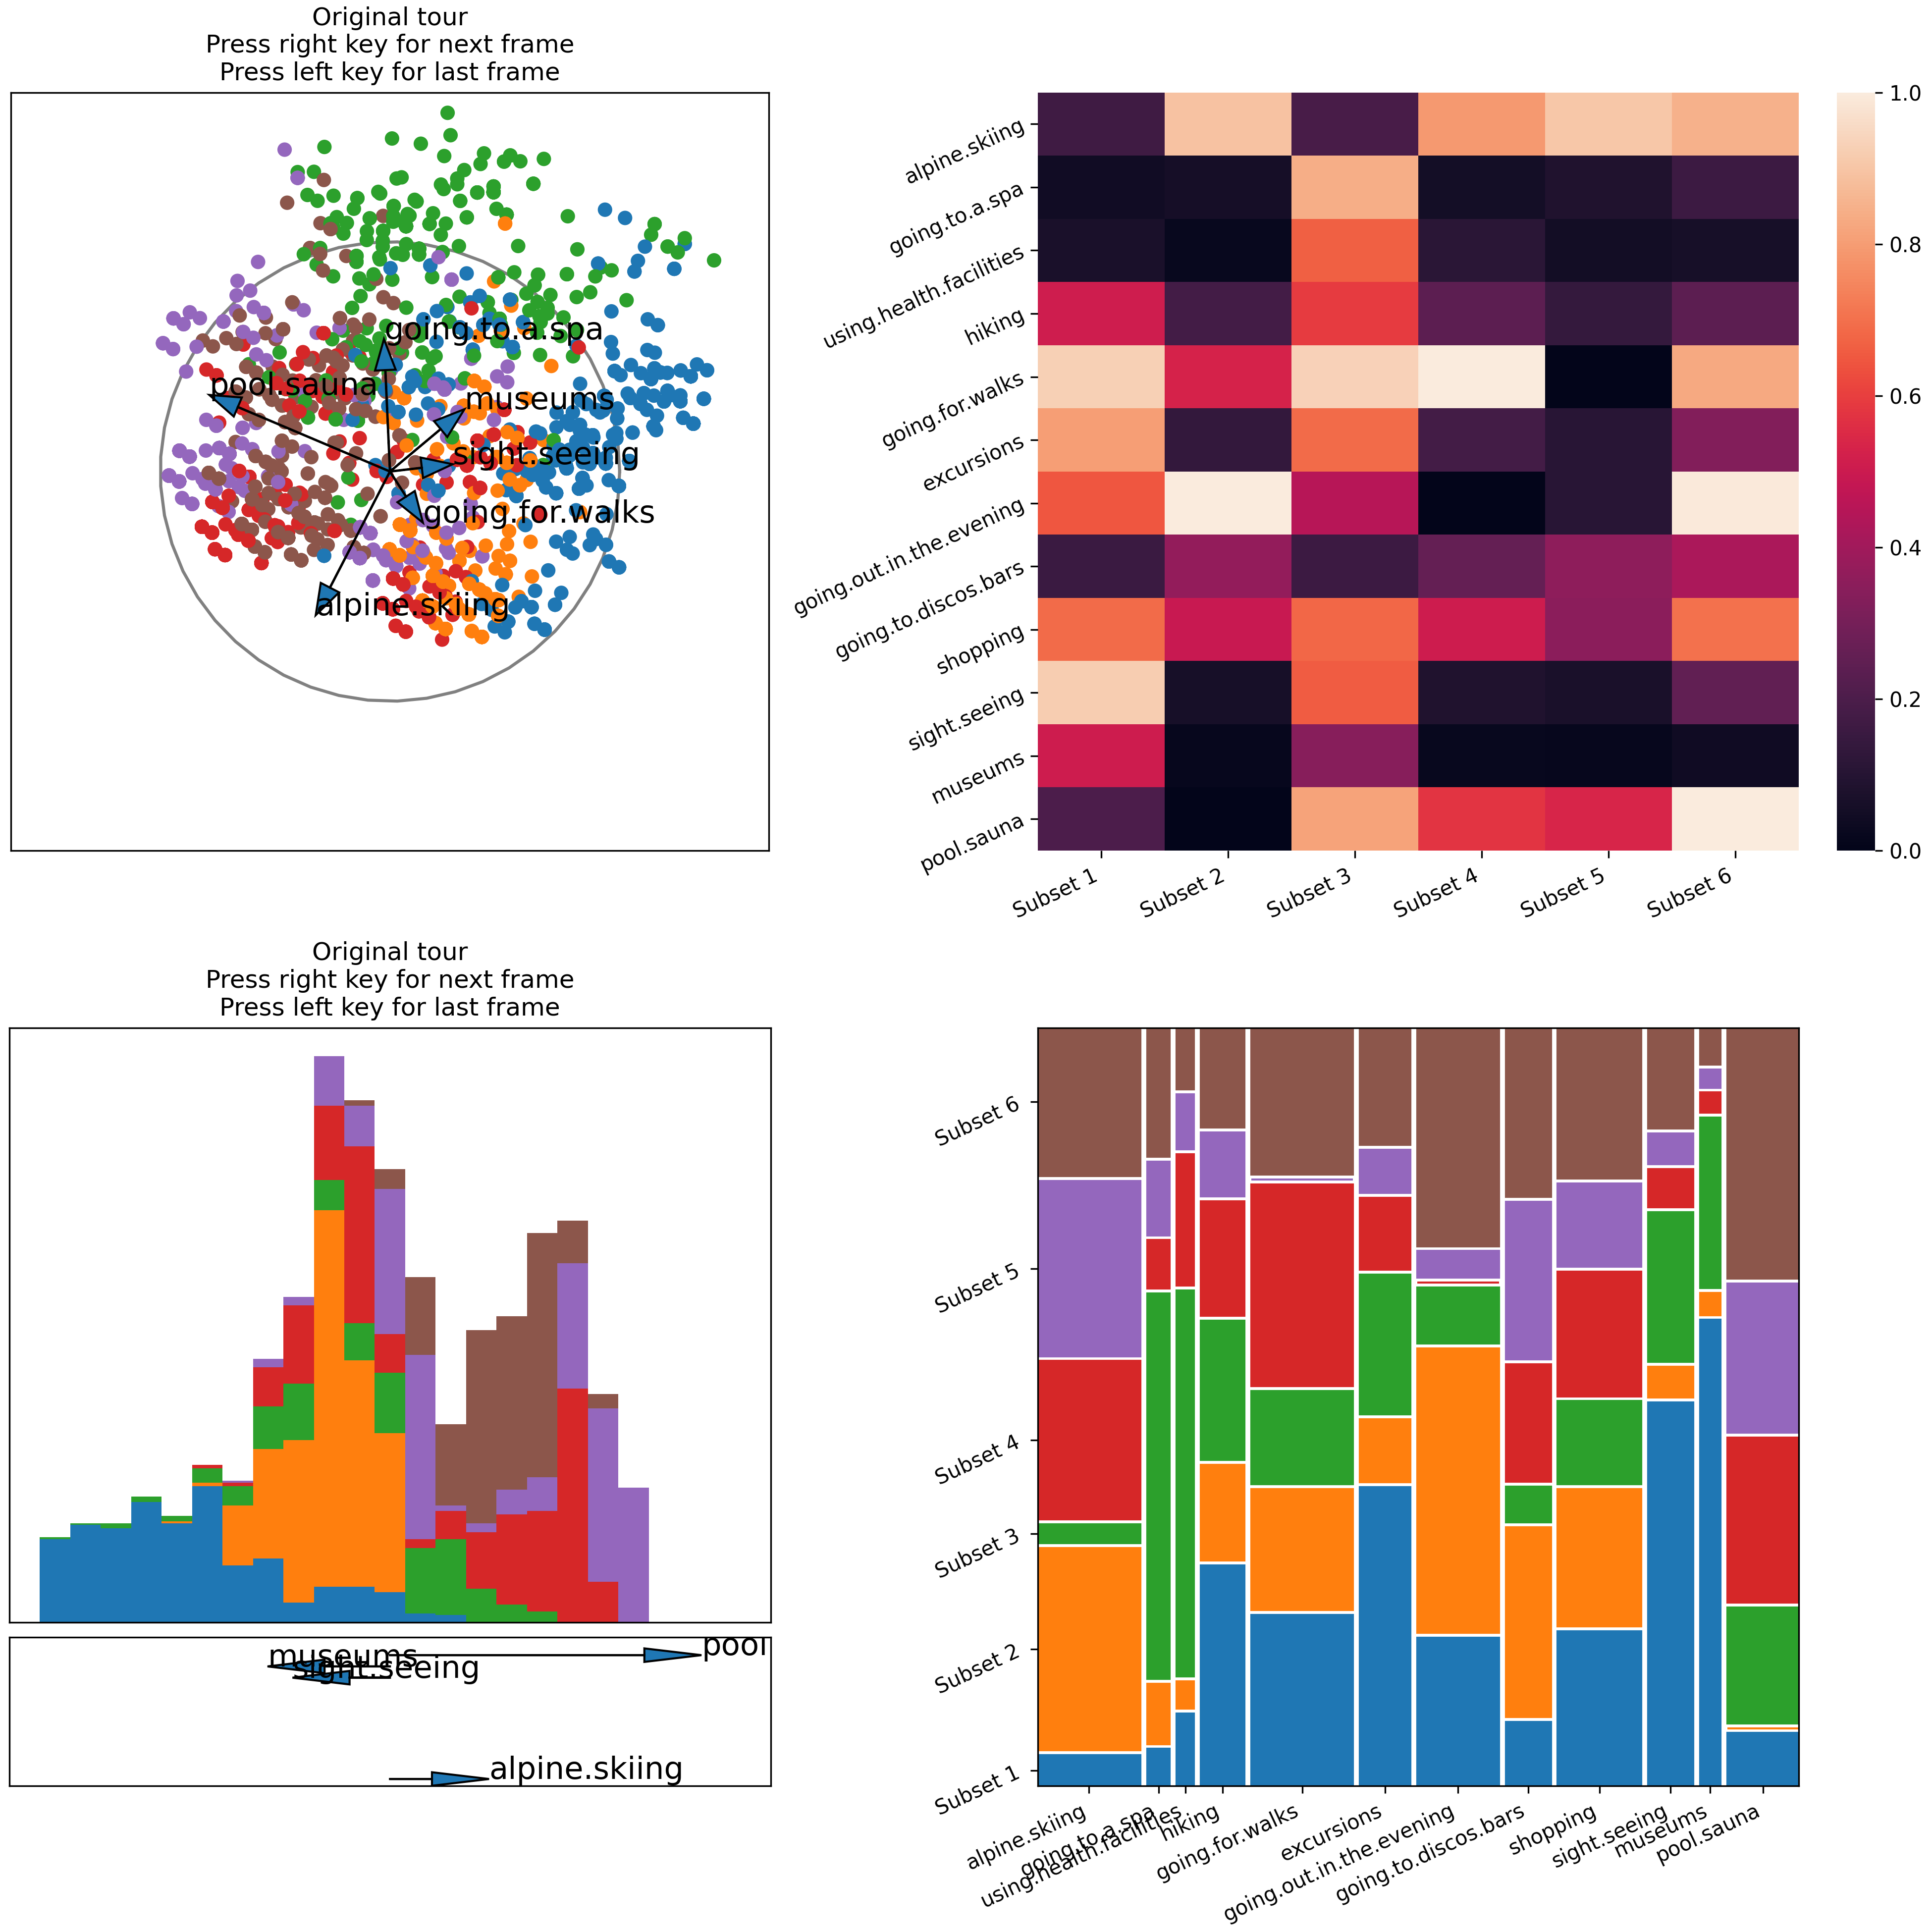
\includegraphics[width=1\textwidth]{winter_cl7_init.png}
    \caption{Top left: 2D tour with the linear discriminant analysis projection pursuit index. Top right: heatmap with the intra-cluster fraction. Bottom left: 1D tour with the linear discriminant analysis projection pursuit index. Bottom right: mosaic plot.}
    \label{fig:winter_cl7_init}
\end{figure}

\begin{itemize}
    \item A 2D tour with the linear discriminant analysis projection pursuit index,
    \item A heatmap displaying the intra-cluster fraction,
    \item A 1D tour with the linear discriminant analysis projection pursuit index, and
    \item A mosaic plot.
\end{itemize}

This setup produces the display shown in Figure \ref{fig:winter_cl7_init}. We can observe that clusters 1 and 3 overlap significantly in the features "sightseeing," "museums," and "going out in the evenings." By highlighting clusters 1 and 3, and adjusting the projection axes, we can confirm that there is indeed overlap between these clusters, as shown in Figure \ref{fig:winter_cl7_pre}.

\begin{figure}[h!]
    \centering
    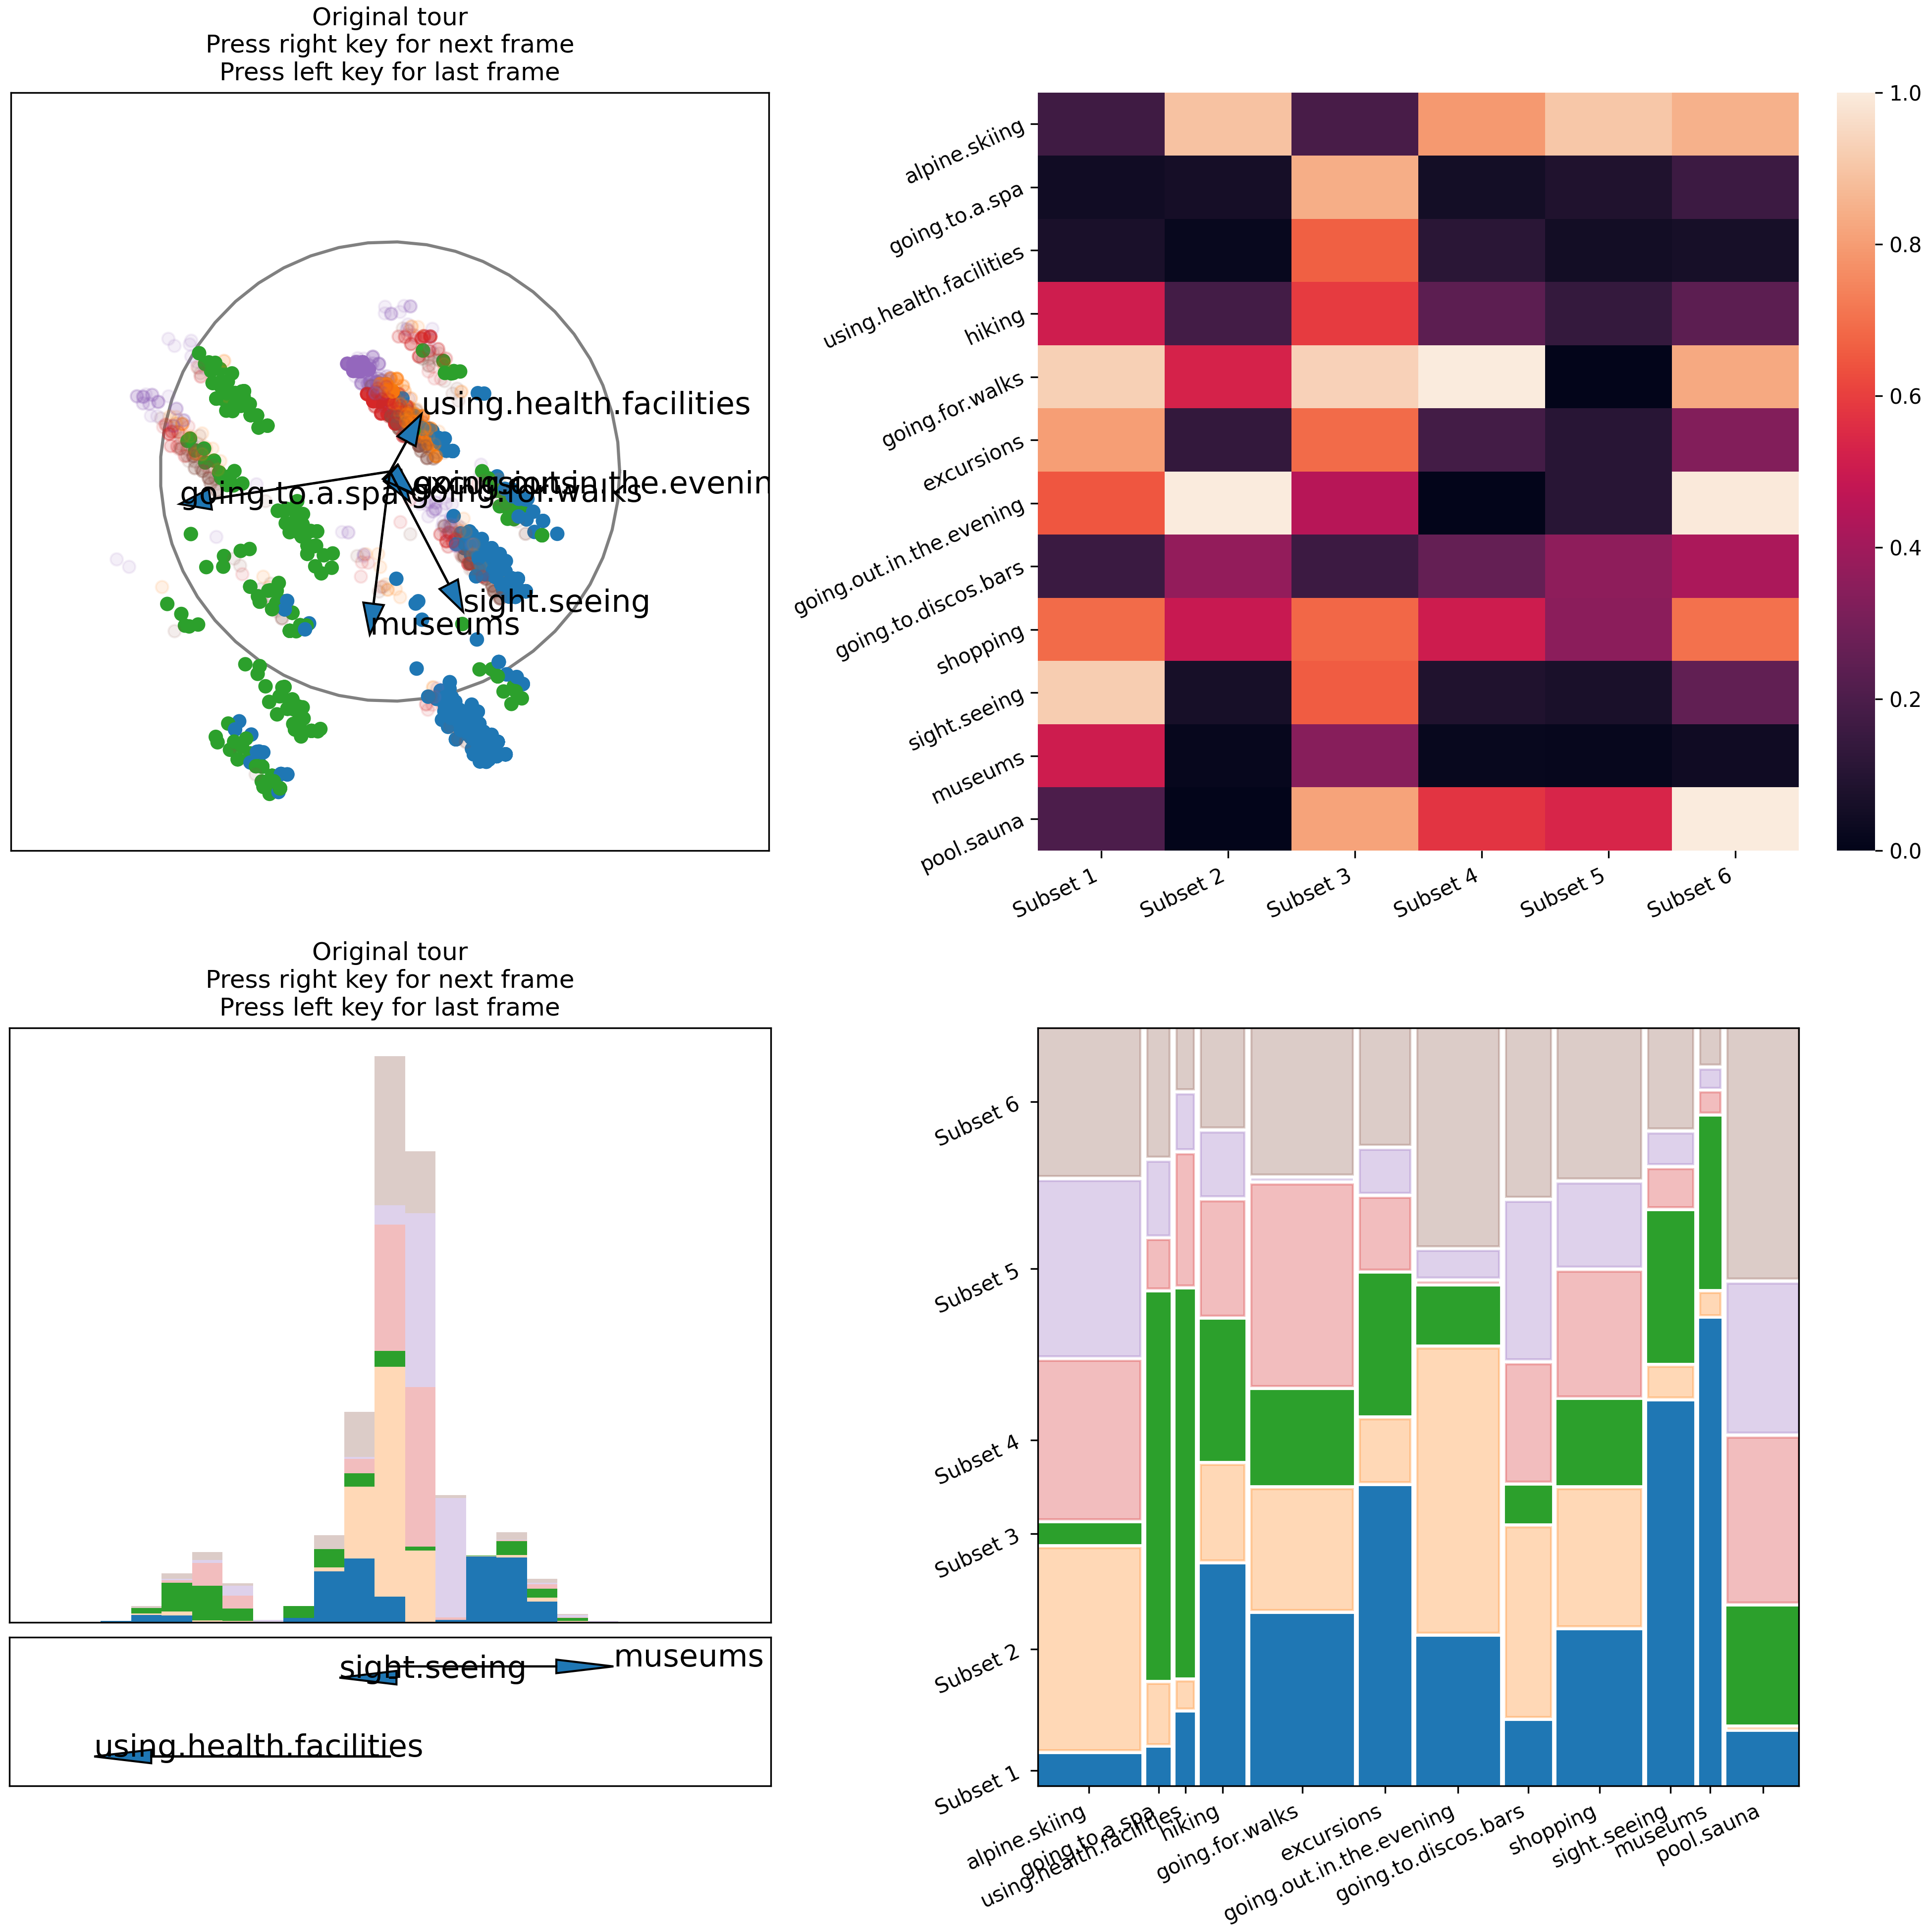
\includegraphics[width=1\textwidth]{winter_cl7_pre.png}
    \caption{Top left: 2D tour with the linear discriminant analysis projection pursuit index. Top right: heatmap with the intra-cluster fraction. Bottom left: 1D tour with the linear discriminant analysis projection pursuit index. Bottom right: mosaic plot.}
    \label{fig:winter_cl7_pre}
\end{figure}

To improve the quality of the k-means solution, we can select the checkmark for subset 7 and manually select the region of overlap. The selected data points will then be shifted to a new cluster: cluster 7. The interface with the newly formed cluster can be seen in Figure \ref{fig:winter_cl7_post}.

\begin{figure}[h!]
    \centering
    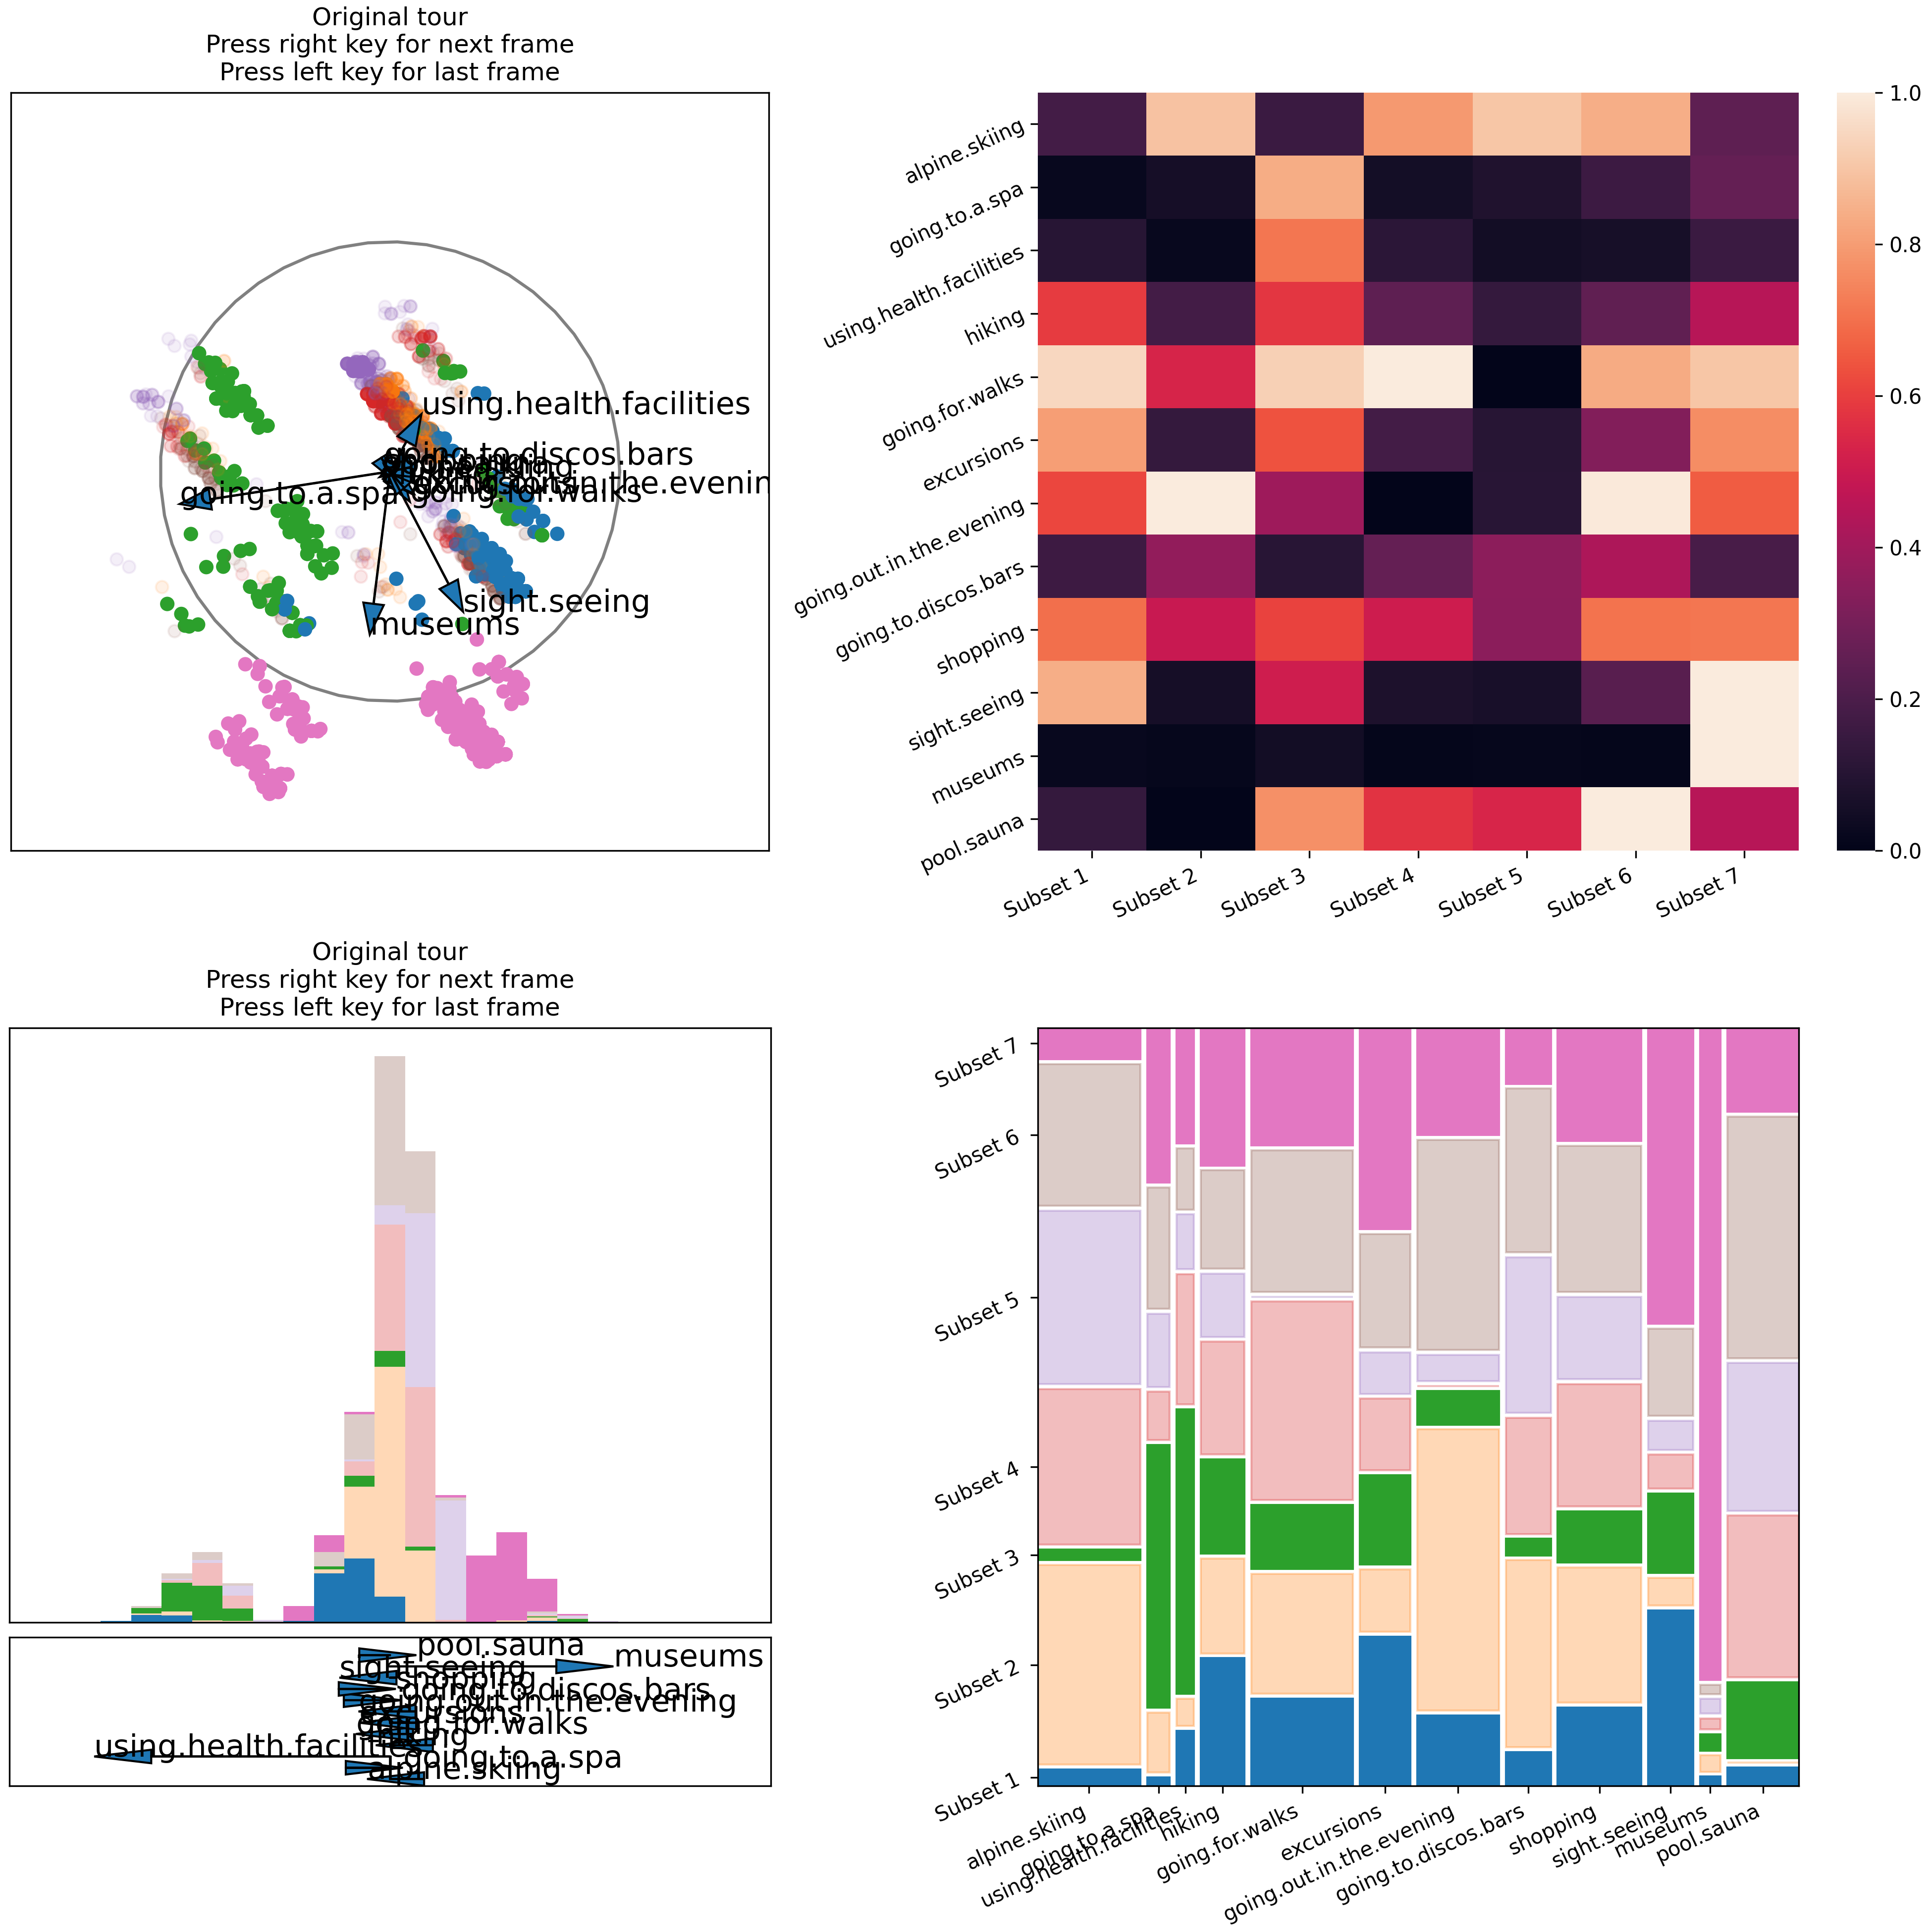
\includegraphics[width=1\textwidth]{winter_cl7_post.png}
    \caption{Top left: 2D tour with the linear discriminant analysis projection pursuit index. Top right: heatmap with the intra-cluster fraction. Bottom left: 1D tour with the linear discriminant analysis projection pursuit index. Bottom right: mosaic plot.}
    \label{fig:winter_cl7_post}
\end{figure}

To assess the quality of the manually enhanced cluster solution, we can compare the silhouette plots of this new solution with those from a k-means solution where \(k = 7\). These silhouette plots are shown in Figure \ref{fig:silhouette_comparison_k7_man}. It is evident that the manually enhanced cluster solution better describes the data compared to the k-means solution with \(k = 7\).

\begin{figure}[h!]
    \centering
    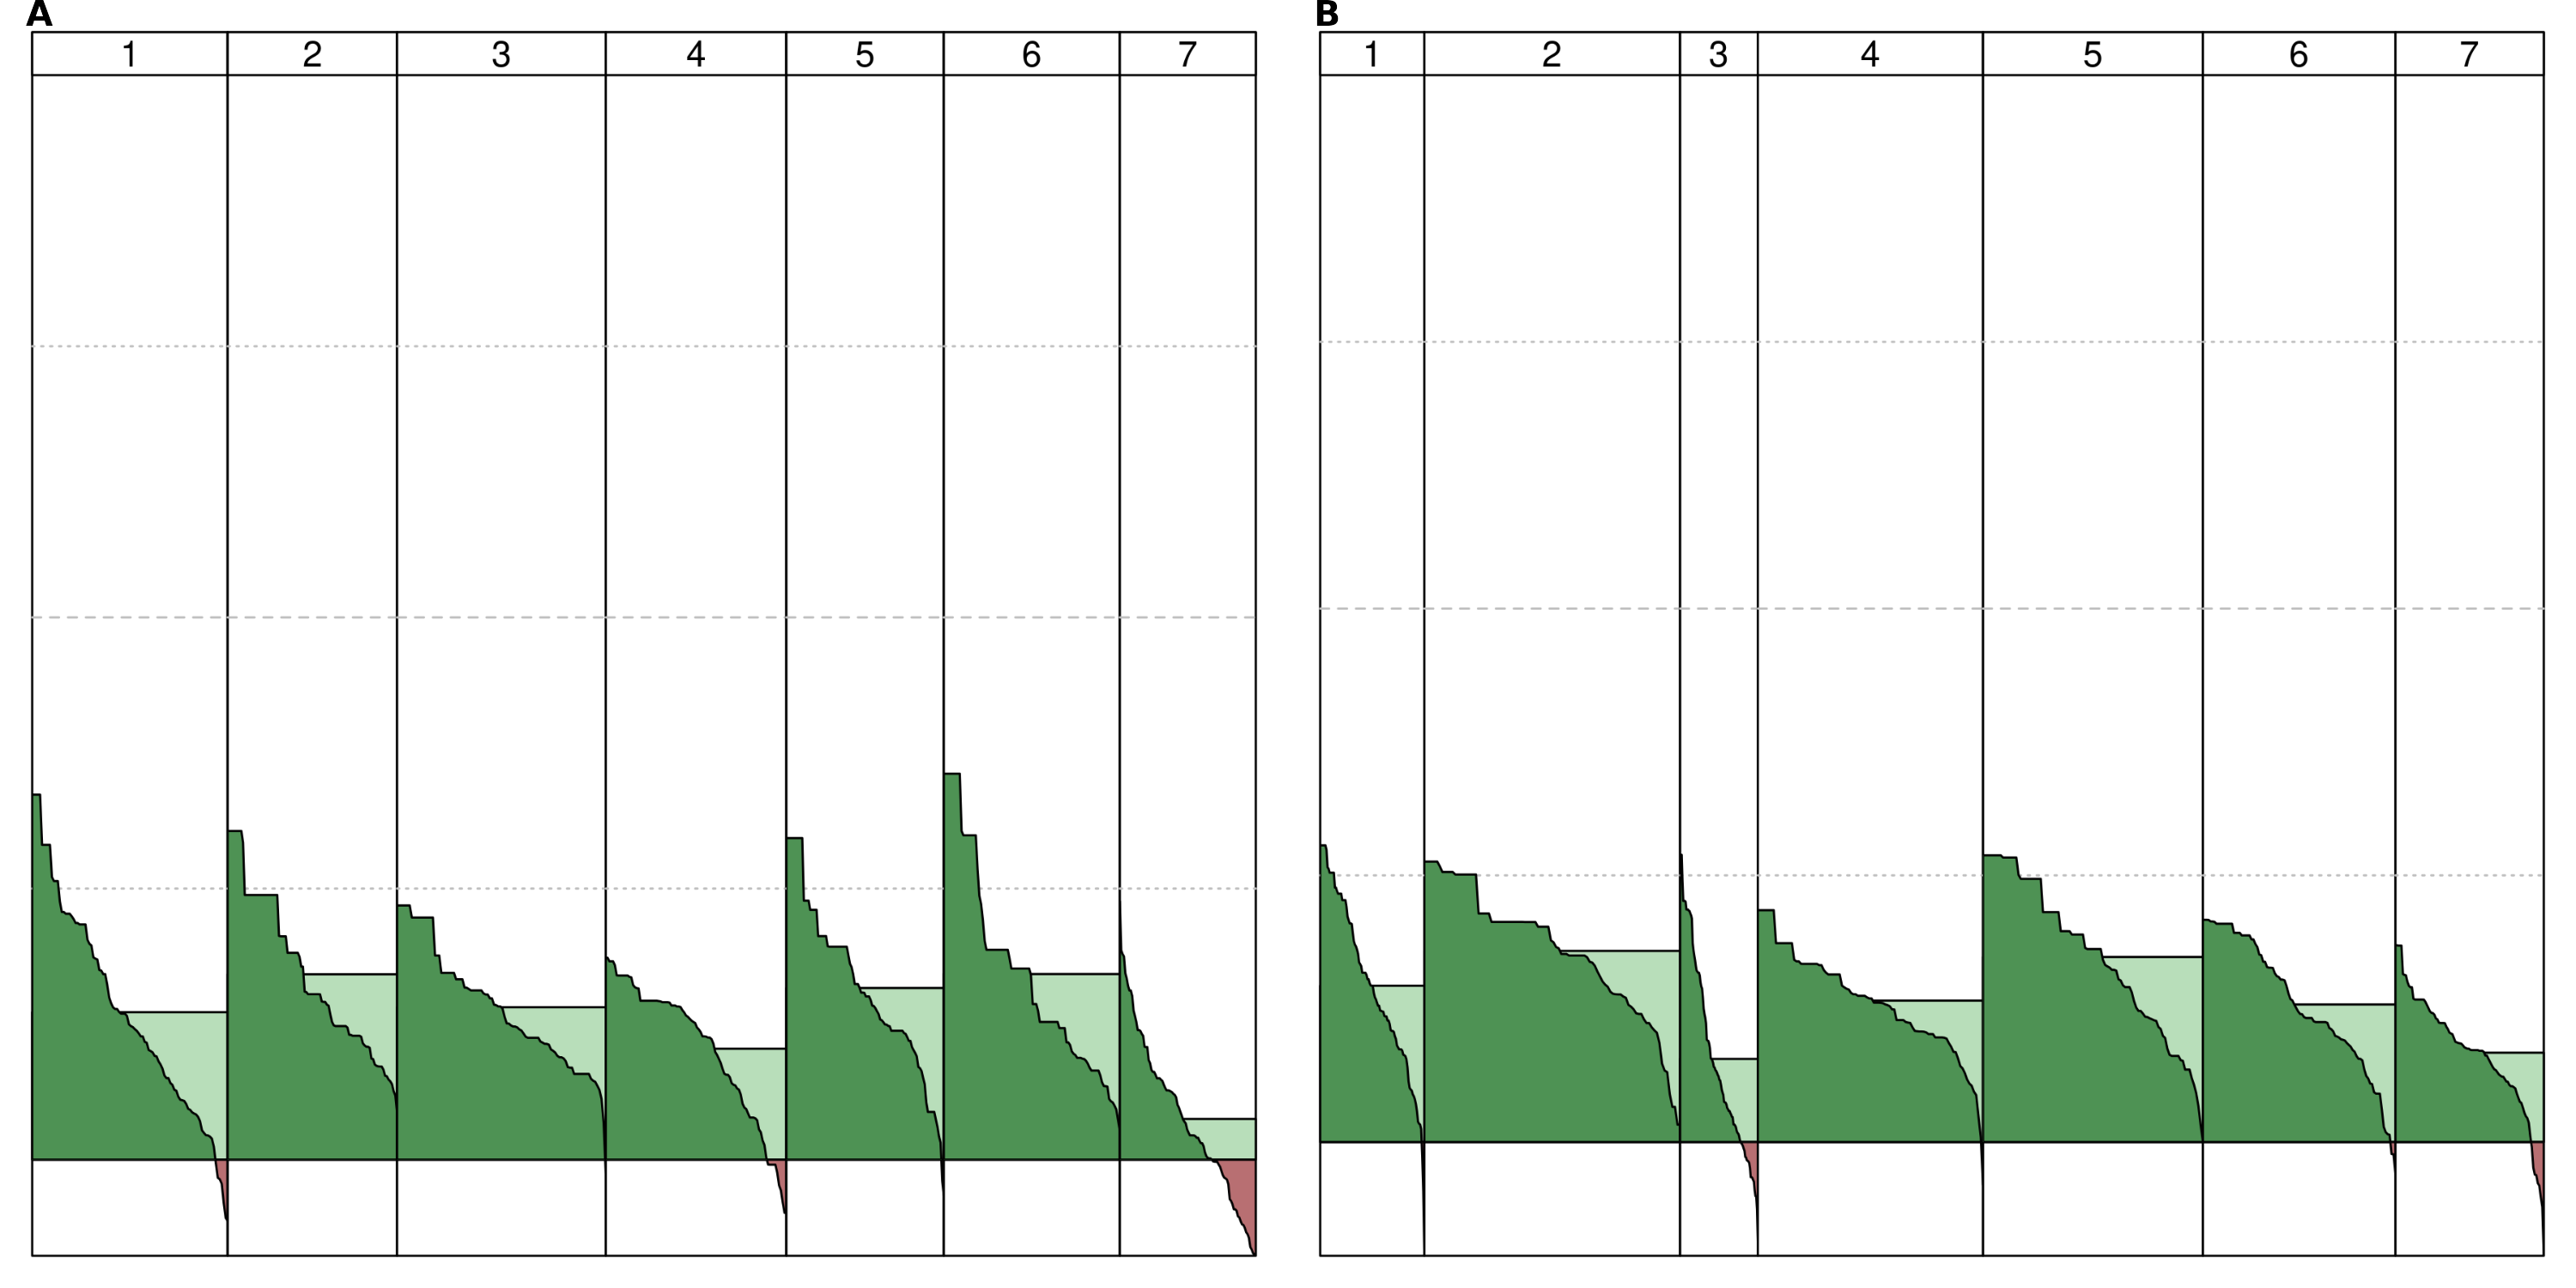
\includegraphics[width=1\textwidth]{silhouette_comparison_k7_man.png}
    \caption{A: Silhouette plot of the k-means solution with \(k=7\). B: Silhouette plot of the manually enhanced k-means solution with \(k=6\).}
    \label{fig:silhouette_comparison_k7_man}
\end{figure}

Additionally, manually enhancing a cluster solution has the advantage of maintaining the base structure of the clustering, whereas clusters in a new k-means solution can be entirely different. Moreover, tourists in cluster 7 now appear primarily interested in cultural activities, such as visiting museums, and not in activities like alpine skiing, going to the spa, using health facilities, or going to discos/bars.


!Note to this section! comparing the average shilouette scores indictes that the original k=6 solutiuon is best, even though in my opinion the plots look better with the manual solution. The scores are:

k=6: 0.1460762

k=7: 0.1336373

k=6 + manual: 0.140716

Let me know what you think


\subsection{Australian Vacation Activities dataset}

The second dataset, the Australian Vacation Activities dataset, includes responses from 1,003 adult Australians who were surveyed through a permission-based internet panel. The survery was conducted in 2007. Participants were asked whether they engaged in 44 specific vacation activities during their most recent vacation within Australia. Similar to the Austrian dataset, responses were binarized: a value of 1 indicates that the participant took part in the activity, while a value of 0 signifies they did not.


\section{Discussion}


\section{Conclusion}

%\bibliographystyle{plainat}
\bibliography{pytourr_references.bib}



\end{document}